For the first problem, we look at the position of a flow particle with a cylinder as obstacle. The results are displayed in the following way. On figure~\ref{fig:c1} one can see the trajectory for different initial positions. The particle never touches the cylinder but they get ever closer as the initial $y\txt{-position}$ gets close to zero.

\begin{figure}[!h]
\centering
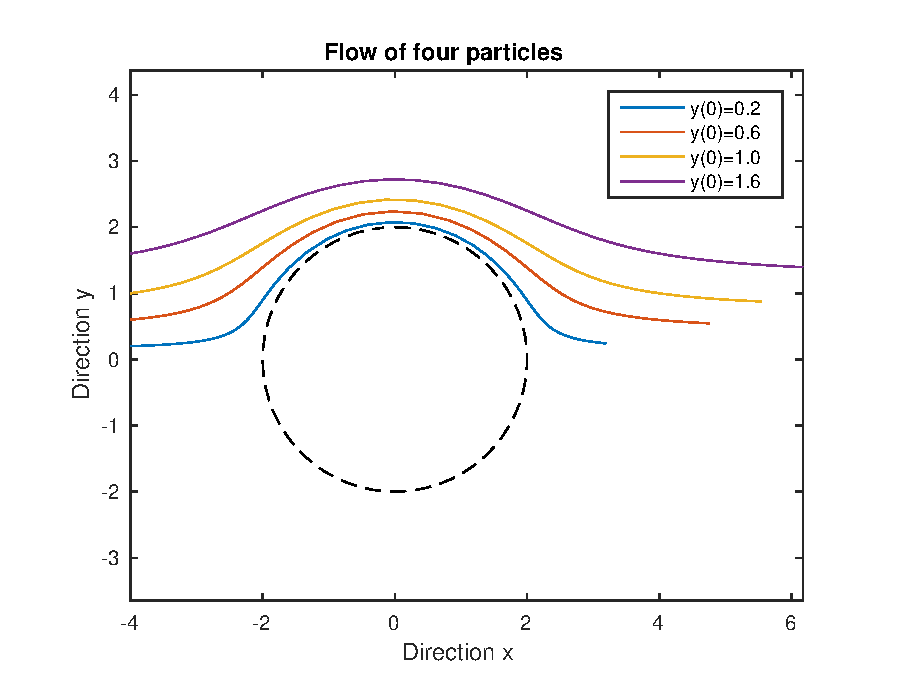
\includegraphics[width = 0.9\textwidth]{./c1.eps}
\caption{Trajectories of the flow in the plane}
\label{fig:c1}
\end{figure}

The second problems is the motion of a particle thrown in the plane. There are two parameters that come into play. The launch angle $\alpha$ and $k$ the air resistance coefficient. We considered $\alpha= 30, 45, 60$ degrees and $k=0.002, 0.065$. For this problem we have one figure for each value of $k$. Each figure shows the motion of the particle for the different launch angles. We see that the launch angle that gives the largest horizontal travelled distance depends on the coefficient k. In the options of the Matlab solver \texttt{ode45}, we specified that the solution $y$ can not become negative (as the ground prevents it).


\begin{figure}[!h]
\centering
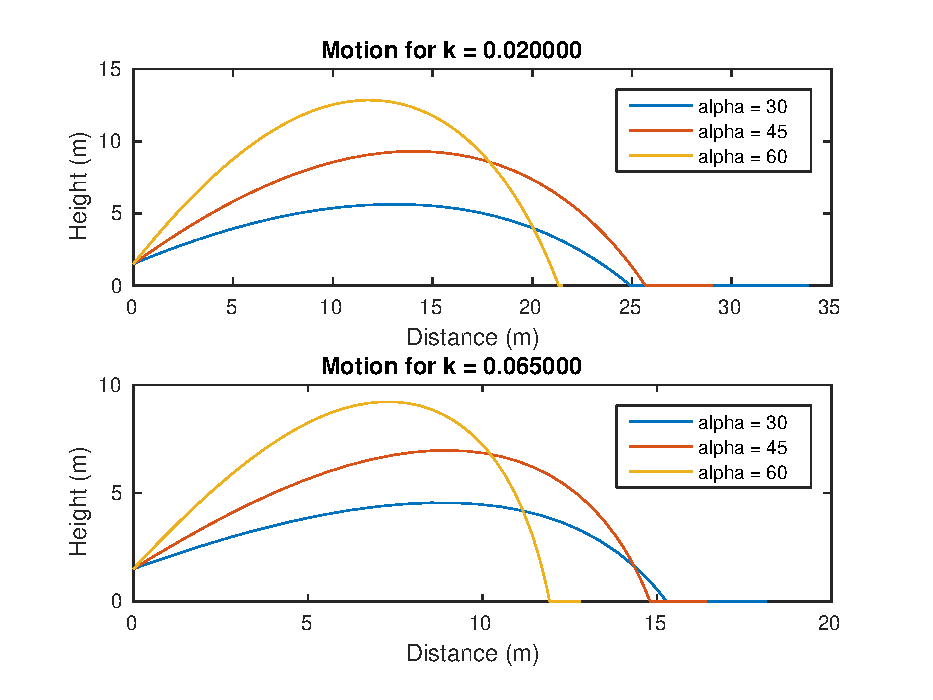
\includegraphics[width = 0.9\textwidth]{./c2.eps}
\caption{Trajectories of the particle in the plane}
\label{fig:c2}
\end{figure}
\FloatBarrier
Below the reader can find our codes for the two problems.
\lstinputlisting{LAB2C1.m}

\lstinputlisting{LAB2C2.m}
